\chapter{Implémentation}
    Le projet est développé en c++ utilisant des notions de programmation modernes.
    Un fichier \textit{stdafx.h} était utilisé. Ce fichier avait pour but de centraliser l'intégralité des fichiers d'en tête du projet. Il était ensuite inclue dans tous les fichiers sources. Ce système permet de précompiler les fichiers d'en-tête. Après discussion avec le client, cette fonctionnalité a été enlevée.

    \section{Implémentation générale}
    \subsection{Problème rencontré}
    Le contexte OpenGL crée par le développeur d'origine du projet était faux. Ça se traduisait au niveau
    de l'application par un plantage d'OpengGL sur certaines cartes graphiques. En particulier sur les processeurs graphiques intégrés. Cette erreur a été très vite corrigée.
   
    \subsection{Portage vers \textit{CMake}}
    Le programme utilisait au départ des scripts de compilations écrit en \textit{Lua} et basés sur le logiciel \textit{Genie}.
    Une des demandes du client était de créer un script de compilation utilisant \textit{CMake}.
    Le \textit{CMake} permet de lancer la compilation du logiciel, il est configuré pour cloner les différentes dépendances. 
    Il permet aussi de générer la documentation du code en utilisant l'outil \textit{Doxygen}.\\
    
    \section{Cartes des hauteurs}
    Comme expliqué dans le chapitre architecture, la carte de hauteur est envoyée sur la carte graphique sous la forme
    d'une texture.\\
    Dans la version de base du projet, seules des cartes de hauteurs sont chargées depuis le disque. Ces images codées sur un
    seul octet signé sont alors converties en flottant et envoyées à la carte graphique. Cette implémentation pose un très gros problème de précision des valeurs, ces dernières entant comprise entre 0 et 255 ne sont pas suffisantes pour représenter
    avec précision une hauteur. C'est-à-dire que la carte de hauteur sera appliquée sur la planète entière mais dès que l'on va zoomer, les valeurs ne seront pas suffisante pour placer avec précision le sommet.
    
    \subsection{Implémentation de base}
    Pour résoudre ce problème, le programme de base charge quatre autres cartes de hauteur avec des niveaux de détails plus élevés. Cependant, cette implémentation créée d'autres problèmes, le plus important est que les différentes textures détaillées nommées \textit{MoonDetail1}, \textit{MoonDetail2} et \textit{MoonHeightDetail1} sont chargées depuis le disque dans le constructeur de la classe Planet. Ce qui casse l'architecture globale du projet, la classe Planet étant une classe abstraite qui se dérive en différents types de planètes tels que Moon ou Earth.
    Cela implique que lorsque la planète terre est créée, les textures détaillées de la lune sont chargées et appliquées.
    Visuellement cela se traduit par l'affichage des cratères de la lune sur la terre.

    L'utilisation des cartes de hauteurs de différents niveaux de détails pose aussi un problème de discontinuité dans le plaquage des textures qui se traduit par des sauts importants dans les hauteurs affichées.\\
     
    \begin{figure}
        \centering
        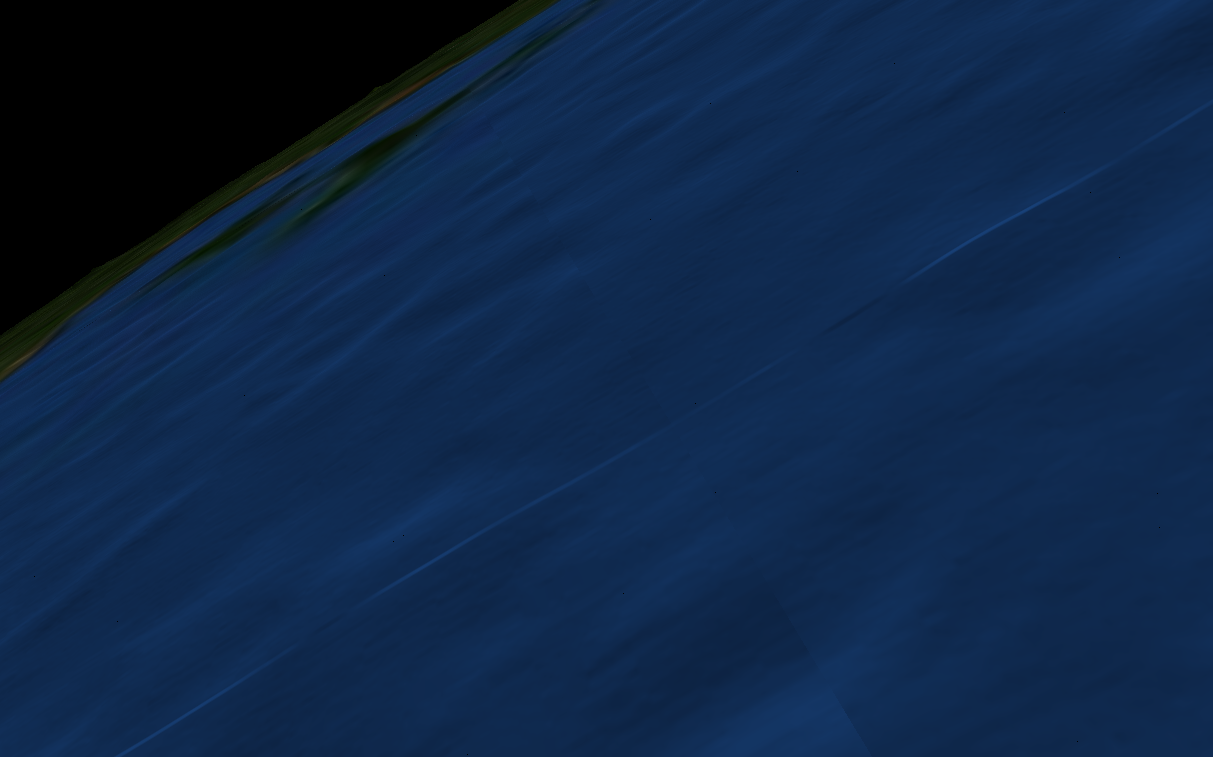
\includegraphics[width=12cm]{img/earth.png}
        \caption{Affichage de la terre}
        \label{fig:earth}
    \end{figure}
    
    
    La figure \ref{fig:earth} présente les deux problèmes majeurs, on peut voir dans l'océan les cratères induits par la texture de la lune. On peut aussi remarquer au centre de l'image une discontinuité.\\
    
    \paragraph{Critique} On peut aussi critiquer l'utilisation de textures chargées depuis le disque car ces dernières, à l'instar d'une génération procédurale passée par des prétraitements et des formats de fichiers avec compression.
    %\textbf{TODO : Peut être éclaicir l'image pour mieux distinger les artéfacts}
    
    \begin{figure}
        \centering
        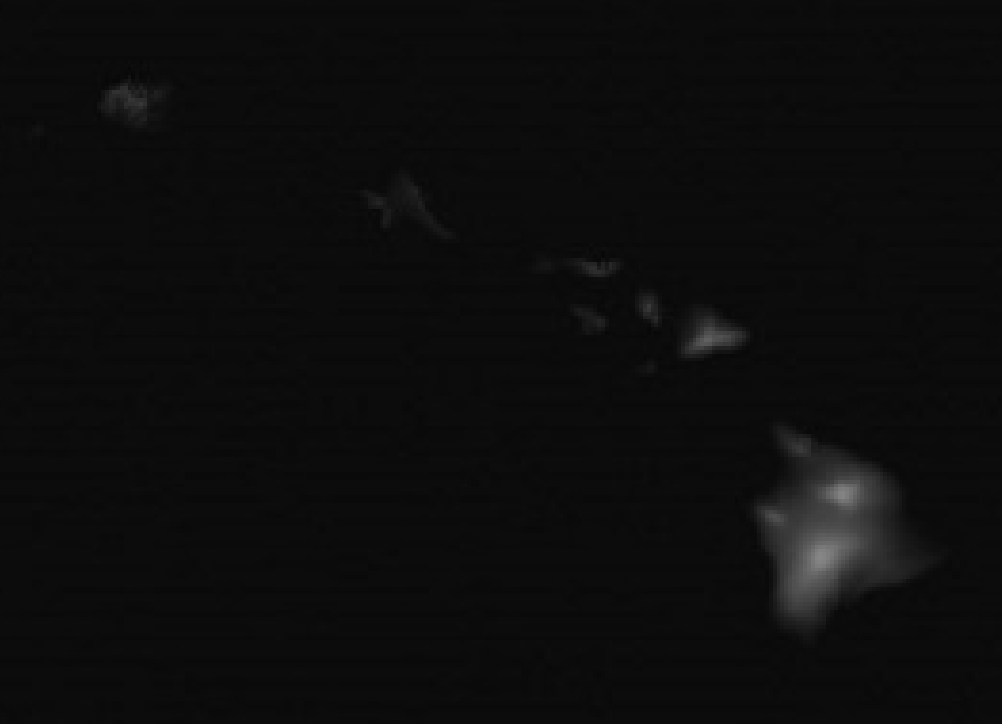
\includegraphics[width=12cm]{img/hawaii.png}
        \caption{Archipel d'Hawaii}
        \label{fig:hawaii}
    \end{figure}
    
    La figure \ref{fig:hawaii} représente l'archipel d'Hawaii extrait de la carte de hauteur de la terre
    (\textit{EarthHeight16k.jpg}). On distingue très clairement des artéfacts dans la partie océan.
    
    \subsection{Travail effectué}
    Une classe Procedural a été écrite, elle permet de créer une planète en utilisant un algorithme de bruit
    sur la texture de la carte de hauteur.
    Des modifications importantes ont été faites dans le code de Texture et dans le shader patch.
    Un nouveau constructeur a été écrit pour prendre en charge ce nouveau type de texture. En effet de 
    base le constructeur reçoit une chaîne de caractères représentant un chemin d'accès sur le disque.
    Ce nouveau constructeur prend quand à lui un tableau à deux dimensions de flottants et sa taille en paramètre.\\
    La méthode $Texture::load$ a aussi été modifiée pour permettre l'envoi de ce tableau directement à la carte graphique.\\
    
    \subsection{Correction des problèmes}
    Le problème subsiste lorsque qu'on charge une image depuis le disque mais lorsque l'on génère procéduralement une image,
    il n'y a pas de conversion vers flottant donc pas de problème. Les données sont directement des flottants dispersés sur toute la gamme [-1;1].\\
    De même, comme des données suffisamment précises sont créées, il n'est plus nécessaire de charger des images supplémentaires. Ce qui corrige aussi les problèmes de discontinuités.\\
    L'image doit cependant être générée avec un algorithme de bruit 3d.\\
    
    
    Actuellement encore un bug subsiste, un dépassement de tampon au sein des pilotes graphiques. 
    Les données étant tous le temps dans
    la même page mémoire, le programme ne plante pas. Cependant, les données pointées lors de ce dépassement étant indéfinis, certains sommets pouvaient avoir une hauteur bien supérieure à la normal. Une solution provisoire était de seuiller les sommets dans le \textit{shader}.\\
    Finalement la solution a été trouvée, le problème était qu'un tableau à deux dimensions était alloué.
    Bien que la fonction d'OpenGL requière une hauteur et une largeur, il faut lui passer un tableau à une dimension. Une explication plus détaillée est faite dans la section \ref{sec:class_texture}
    
   \section{Génération du maillage}	% Explication de triangulator.
  % icosaèdre ?
  % triangulator ?
  % structure de données
	\subsection{Icosaèdre}
	\label{subsec:icosaèdre}
	
	Il existe plusieurs manières de générer un maillage de planète, la méthode utilisée ici
	se base sur un icosaèdre, une forme géométrique composée de douze sommets de base et 
	de vingt faces triangulaire. Chaque face étant un triangle équilatéral de taille identique.
	
	Pour se faire il est nécessaire d'utiliser le nombre d'or $\Phi = \frac{(1+\sqrt(5)}{2}$ , qui est le seul rapport permettant de construire le plus petit deltaèdre ( polyèdre dont les faces sont toutes des triangles équilatéraux).
	
	La méthode utilisée pour former les triangles équilatéraux (et donc l'icosaèdre) et de se servir de 3 plans respectant les proportions du nombre d'or, qui se coupe en leur centre. En reliant les 12 sommets possibles, on va ainsi former les 20 faces de notre icosaèdre, comme on peut l'observer sur la figure \ref{fig:plans-icosaèdre}.
	
	\begin{figure}[H]
        \centerline{
            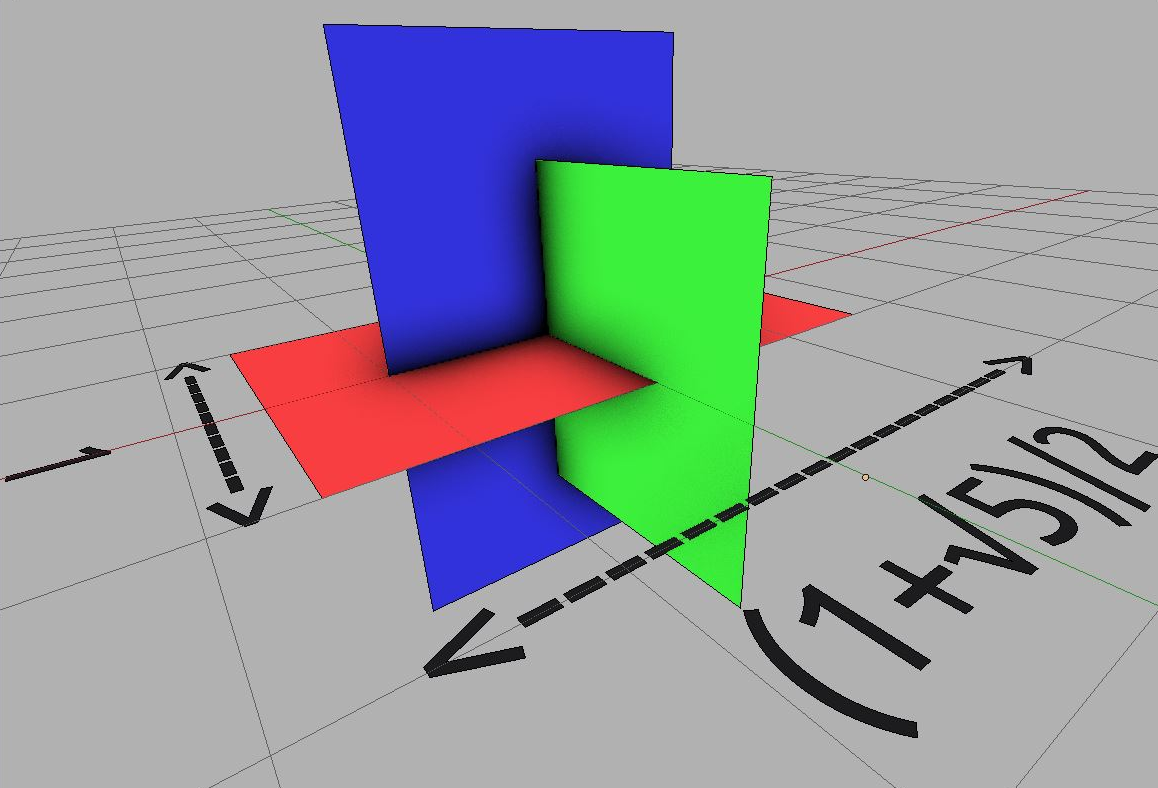
\includegraphics[height=4cm,width=4.5cm]{img/3plans.png}
            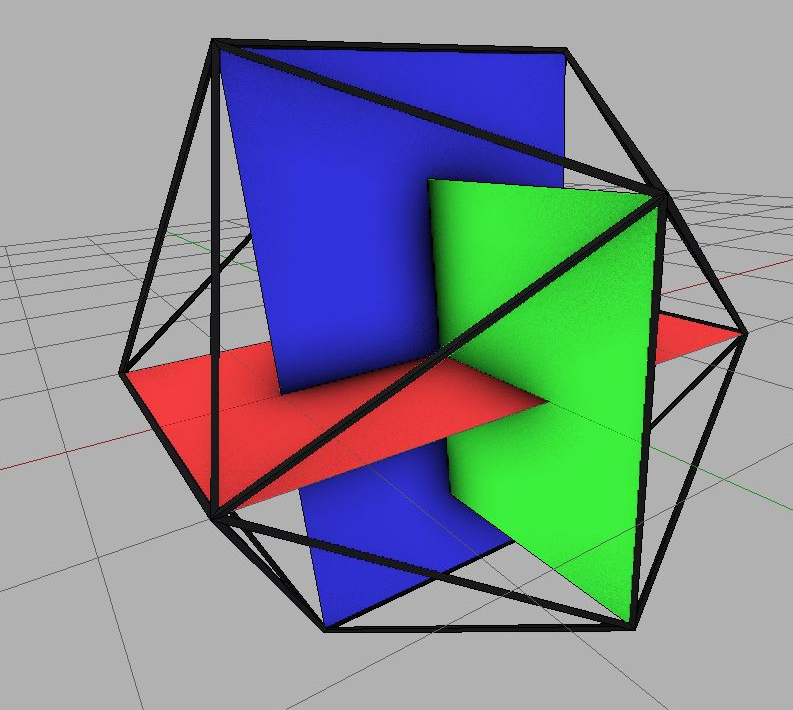
\includegraphics[height=4cm,width=4cm]{img/3plans2.png}}
        \caption{Formation de l'icosaèdre \protect\footnotemark}
        \label{fig:plans-icosaèdre}
	\end{figure}
	\footnotetext{Extrait de \url{http://robert-lindner.com/img/blog/planet_renderer/week5-6/researchPaper.pdf}, dernier accès Mars 2018}
	
	
	% Parler de la generation avec le nombre d'or
	
	La génération du maillage et l'entièreté de la partie LOD de l'algorithme se font dans la classe Triangulator. L'arbre de données est implémenté avec la méthode des flux du CDLOD (StreamingCDLOD), dont les avantages ont été expliqué précédemment.
	
	L'implémentation ici ne suit pas entièrement le standard du \textit{StreamingLOD}, il a été expliqué que l'algorithme peut conserver les parties qui restent dans le champs de vision. Ici l'intégralité de l'arbre est régénéré à chaque tour de boucle. Cependant dans un contexte de visualisation simple les gains de performances engendrés par de telles optimisations sont négligeables.
	
	Pour accélérer les temps d'accès mémoire, les distances avec les différents triangles sont conservées
	dans un tableau. \\

	Dans l'arbre, chaque n\oe{}ud possède trois positions correspondant aux trois points du triangle,
	ainsi que quatre pointeurs vers les niveaux suivants.
	D'autres informations sont stockées comme un pointeur vers son parent, le niveau actuel du
	n\oe{}ud dans l'arbre ou encore un drapeau correspondant au type du n\oe{}ud.
	Le drapeau sous forme d'un \emph{enum} permet de distinguer le n\oe{}ud qui sont a l'intérieur de l'arbre de ceux
	qui ne le sont pas. Il permet aussi de renseigner si le n\oe{}ud est une feuille.
		
	Pour chaque triangle, on commence par tester si le triangle est visible, c'est-à-dire s'il est
	présent à l'intérieur du cône de vision de la caméra. Si c'est le cas, on prend le centre de chaque
	arrête du triangle l'on recommence de manière récursive tans qu'une subdivision est nécessaire.
	C'est-à-dire tans que le n\oe{}ud contenant le triangle n'est pas une feuille. Dans le cas contraire,
	
	
    \begin{figure}[!ht]
        \centerline{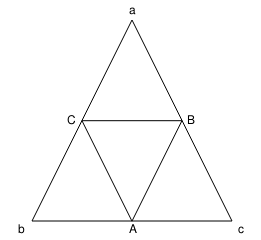
\includegraphics[width=5cm]{img/TriangleSplit.png}}
        \caption{Division}
        \label{fig:TriangleSplit}
    \end{figure}
	
	On peut se rendre compte de la découpe du triangle en quatre plus petit dans la figure 
	\ref{fig:TriangleSplit}.
	Les appels récursifs se font dans l'ordre aBC, AbC, ABc et enfin le triangle du milieu ABC.\\
	
	La méthode SplitHeuristic permet en fonction de trois coordonnées représentant un triangle 
	et du niveau d'établir si ce triangle est dans le cône de vision ou non et de retourner le bon drapeau.
	Les méthodes permettant de déterminer si le cône de vision contient un triangle sont définies dans
	la classe Frustum.
	
  \section{Application du morphing}
  L'algorithme de génération du maillage utilisant le morphing est développé dans la classe \textit{Patch}.\\ 
  
  Le mécanisme du \textit{Patch} est décomposé en deux structures différentes,
  \textit{PatchVertex}, \textit{PatchInstance} et une classe \textit{Patch}.\\
 
  La structure \textit{PatchVertex} permet de stocker les informations relatives à un sommet tel que ça position, codé dans un vecteur de taille 3 et le \textit{morphing}, codé dans un vecteur de taille 2. Ces informations sont ensuite envoyées à la carte graphique.
  
  \textbf{TODO PatchInstance}\\
  
  Il se base sur deux listes appelées m\_Vertices et m\_Indices qui permettent respectivement de stocker des structures \textit{PatchVertex} et des entiers signés.\\
  
  Les informations de positions stockées dans la liste sont envoyées à la carte graphique et permettent de positionner le sommet dans les trois dimensions.\\
  
  La figure \ref{fig:morphTri} représente les transitions du \textit{morphing} lors de l'augmentation du niveau de détails de la zone. Le fonctionnement reste assez semblable à celle expliqué dans la section morphing \ref{subsec:morphing} mais est ici appliqué sur des triangles.
  	
\begin{figure}[H]
    \centering
    \begin{subfigure}[b]{0.17\textwidth}
       \centering 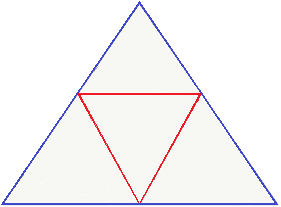
\includegraphics[width=\textwidth,height=2.25cm]{img/morph5.png}
       \caption{}\label{subfig:morph5}
    \end{subfigure}
    ~ 
    \begin{subfigure}[b]{0.17\textwidth}
       \centering 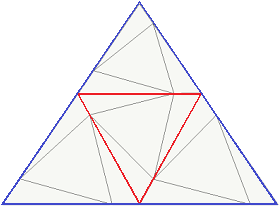
\includegraphics[width=\textwidth,height=2.3cm]{img/morph4.png}
       \caption{}\label{subfig:morph4}
    \end{subfigure}
    ~
    \begin{subfigure}[b]{0.17\textwidth}
       \centering 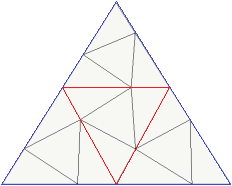
\includegraphics[width=\textwidth,height=2.3cm]{img/morph3.png}
       \caption{}\label{subfig:morph3}
    \end{subfigure}
    ~
    \begin{subfigure}[b]{0.16\textwidth}
       \centering 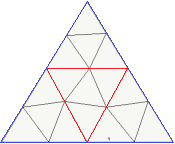
\includegraphics[width=\textwidth,height=2.3cm]{img/morph2.png}
       \caption{}\label{subfig:morph2}
    \end{subfigure}
     ~
    \begin{subfigure}[b]{0.16\textwidth}
       \centering 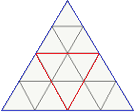
\includegraphics[width=\textwidth,height=2.3cm]{img/morph1.png}
       \caption{}\label{subfig:morph1}
    \end{subfigure}
    \caption{Morph sur des triangles}\label{fig:morphTri}
\end{figure}

    Dans la figure \ref{subfig:morph5}, le triangle Bleu est déjà subdivisé en quatre triangles, et a donc déjà été augmenté en niveau de détails.
    Lorsque l'on change de niveau de détails, chaque triangle concerné est divisé en quatre nouveaux triangles ce qui correspond à l'ajout de trois nouveaux sommets. Ces nouveaux sommets ont tous d'abord la même position que les trois anciens, il reste à la même hauteur que la face, c'est-à-dire qu'ils se déplacent en suivant les arêtes du triangle parent jusqu'au milieu de ce dernier.
    Les figures \ref{subfig:morph4}, \ref{subfig:morph3}et \ref{subfig:morph2} représentent le déplacement des sommets, permettant ainsi d'obtenir le triangle Bleu final, à un troisième niveau de détails visibles dans la figure \ref{subfig:morph1}.\\
    
    Les sommets créées sont ainsi relatifs au triangle et leur position est représentée en deux dimensions sur le même plan.
  
  Ces informations sont stockées dans le vecteur de taille deux dans la structure \textit{PatchVertex}.\\
  
  
  
  
  \section{Frustum}
  
  Comme dit dans la partie architecture, le frustum a pour but d'éliminer les triangles qui ne sont pas présent danss le cône de vision de la caméra.\\
  La figure \ref{fig:culling} représente ce que voit la caméra (matérialisée par la pointe du cône).
  
  \begin{figure}
  \centering
  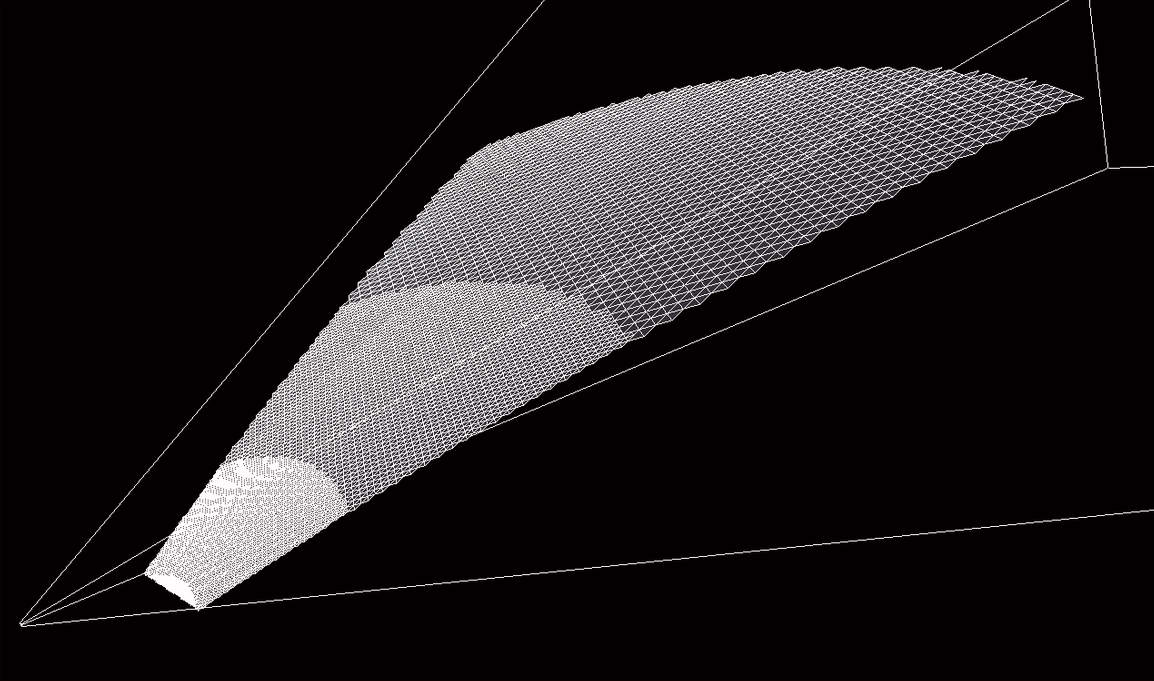
\includegraphics[width=10cm]{img/culling.png}
  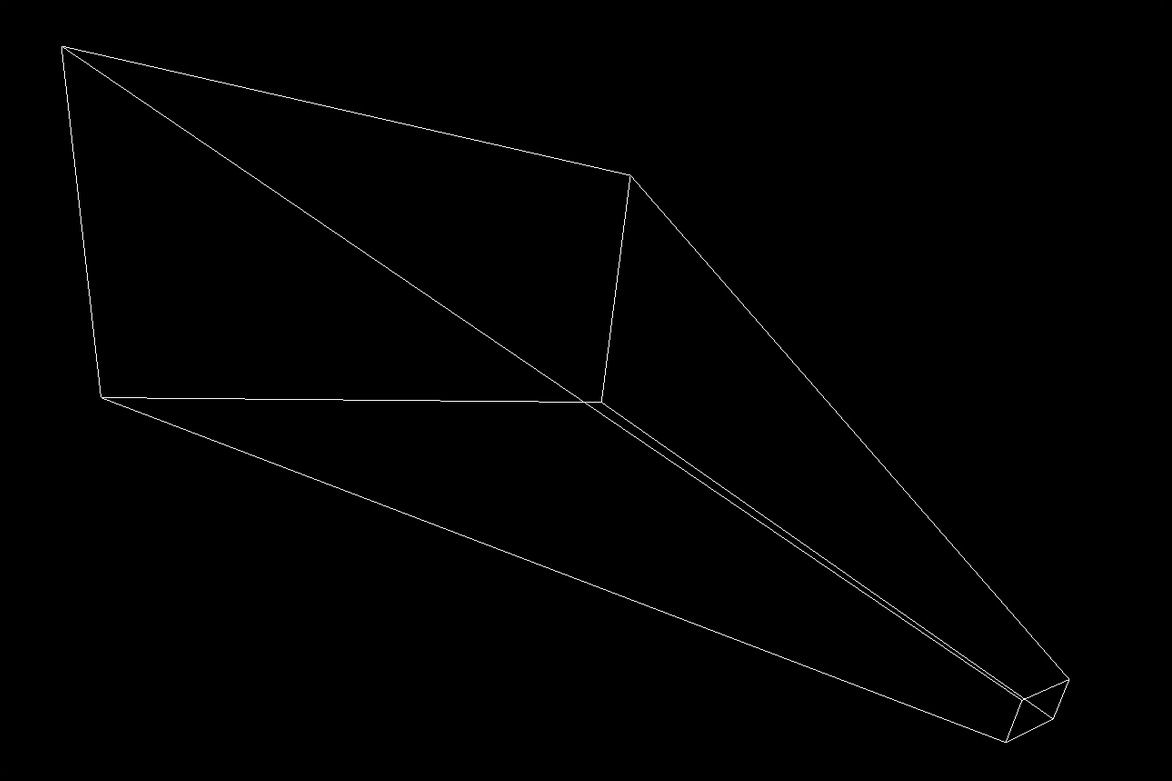
\includegraphics[width=10cm]{img/frustumbox.png}
  \caption{Cône de vision de la caméra \protect\footnotemark}
  \label{fig:culling}
  \end{figure}

  \footnotetext{Extrait de \url{http://robert-lindner.com/img/blog/planet_renderer/week5-6/researchPaper.pdf}, dernier accès Mars 2018}
 
  Le \textit{frustum} est construit autour de six plans différents, quatre représentants les quatre côtés du cône et deux représentants le plan le plus proche et le plan le plus loin.
  On peut voir la structure géométrique du cône de vision dans la figure \ref{fig:culling}
  
  Ces plans sont calculés en fonction de l'angle de vue, de la taille de la fenêtre et des plans \textit{near} et \textit{far}.
  
  \section{Génération de la carte de hauteur}
  
  Dans le code d'origine, les cartes de hauteur étaient chargées depuis le disque. Nous avons développé un nouveau type de planète héritée de \textit{Planet} qui permet de générer une planète avec plusieurs types de bruits différents.
  
  Le processus de création de la texture de bruit se base sur une structure contenant les différents paramètres du bruit.
  Chaque bruit étant spécifique, certain nécessite plus de paramètre que d'autres, par exemple un bruit de \textit{simplex} classique à besoin uniquement d'une taille alors qu'un bruit
  de simplex de type \textit{flow noise} utilise d'autres paramètres comme par exemple un octave. 
  
  \section{Gestion des arguments}
  Nous avons rajouté un système permettant de récupérer et de traiter les valeurs d'entrées du programme.
  Pour cela a été créé une classe \textit{ArgvParser}. Cette dernière est créée grâce aux variables \textit{argc} et \textit{argv}. 
  Cette classe ne gère pas le fait qu'aucun argument ne soit renseigné en entrée. Il faut au préalable s'assurer que \textit{argc} soit strictement supérieur à 1. Ce que l'on fait dans la fonction \textit{main}.\\
  
  \subsection{Classe ArgvParser}
  
  Le but de la classe \textit{ArgvParser} est de récupérer chaque entré de \textit{argv}, les diviser en deux en fonction du caractère "=" et de stocker les deux chaînes de caractères résultants dans un tableau dynamic de deux-uplets (\textit{tuple}.\\
  
  Par exemple avec une entrée "--width=100", un deux-uplets contenant "--width" et "100" est créée et est stocké.\\
  Si une entrée ne contient pas de "=", par exemple "--help" un deux-uplets est créé, avec "--help" et "true" comme valeur. La valeur par défaut lorsque l'on ne trouve pas de "=" est "true".
  Un autre système avait été mis en place à l'origine. Le concept était d'utiliser des paramètres optionnels
  avec la classe \textit{optionnal} de la bibliothèque standard mais ce système a été standardisé en \textit{C++17} et n'est pas disponible dans la version que l'on utilise. Un exemple de l'utilisation de ce système est renseigné en annexe, 
  
  Des méthodes \textit{GetCmdInt}, \textit{GetCmdFloat} et \textit{GetCmdBool} permettent ensuite de récupérer les valeurs correspondant aux arguments.
  
  \lstset{language=C++}
  \begin{lstlisting}
     int main(int argc, char** argv){
        if (argc <= 1)  return -1;
        
        ArgvParser argvParser (argc, argv);
        
        unsigned int width = 0;
        argvParser.GetCmdInt<unsigned int>("--width", &width);
     }
  \end{lstlisting}
  
   \subsubsection{GetCmd*}
    Les méthodes \textit{GetCmdInt}, \textit{GetCmdFloat} et \textit{GetCmdBool} permettent de récupérer la valeur définie après le égale et de la stocker respectivement dans un entier, flottant et booléen.\\
    
    La méthode \textit{GetCmdInt} utilise de la généricité pour permettre de choisir entre un entier signé et non signé. L'utilisation des entiers non signés n'est cependant pas utilisée.\\
    
    La méthode \textit{GetCmdInt} fonctionne uniquement si le type générique renseigné est \textit{int} ou \textit{unsigned int}. Cette limitation est renseignée dans la documentation de la méthode.
    
  \subsubsection{Limitation}
    
    La classe \textit{ArgvParser} ne gère pas les cas où l'utilisateur renseigne un chiffre négatif alors que le programme attend un chiffre positif. Par exemple la sélection d'une taille de texture négative
    n'est pas traitée à ce niveau. Mais gérée au niveau de la création de la planète dans la classe \textit{Scene}.
  
  \section{Création de la planète}
  Une classe \textit{ProceduralPlanet} a été écrite, elle permet conjointement avec la classe \textit{Scene} et \textit{Texture} de créer une texture en fonction des arguments d'entrer du programme.
  
  \subsection{Classe Texture}
  \label{sec:class_texture}
  La classe Texture permet de charger une texture depuis le disque, de la lier à \textit{OpenGL} pour l'utiliser dans les \textit{shaders}.\\
  
  Cette classe a été modifiée pour pouvoir accepter une pointeur sur une texture déjà existante. 
  La difficulté est de correctement configurer OpenGL pour envoyer des données correctes. Les données dont des flottants codés sur 32bit (GL\_32F).\\
  Nous utilisons la fonction \textit{glPixelStorei(GL\_UNPACK\_ALIGNMENT, 1)} pour préciser que les données envoyées à OpenGL sont contiguës. D'après le standard OpenGL cette fonction est nécessaire mais 
  nous n'avons pas trouvé de différences selon la valeur renseignée.
  
  \subsection{Classe ProceduralPlanet}
    \label{sec::ProceduralPlanet}
  Une structure \textit{Properties} est définie à l'intérieur de la classe \textit{ProceduralPlanet}. Elle permet de faire passer les différents paramètres que chaque bruit. 
  Comme certain bruit utilise plus de paramètre que d'autres, par exemple le bruit \textit{FLOW_NOISE} utilise un paramètre de plus que \textit{SIMPLEX}. Pour pouvoir faire passer des structures de tailles variables à \textit{ProceduralPlanet}, il suffit de faire hériter les nouvelles structures de \textit{Properties}, de les créer et de les convertir vers le parent. Ensuite, la structure est passé par pointeur au constructeur de \textit{ProceduralPlanet} et reconvertie. Le code d'exemple ci-dessous montre la procédure.\\
  

  \section{Classe Scene}
  Comme vue dans la partie \ref{sec::ProceduralPlanet}, une structure correspondant au bruit voulu est créé,
  elle est ensuite passé sous forme de pointer à la construction de la planète.\\
  
  Le code de création de la fenêtre était à l'origine dans le constructeur, il a été déplacé dans une méthode dédiée \textit{CreatePlanetFromArgs}. Une méthode \textit{check_value} a aussi été écrite, elle permet de mettre une valeur par défaut dans la variable si cette dernière est égale à une valeur de comparaison. On peut voir que dans l'exemple \ref{fig:code_scene} qu'une structure \textit{FlowNoiseProperties} est créée, elle hérite de \textit{Properties} et est la seule à posséder une
  donnée membre \textit{angle}. La structure est ensuite convertie en \textit{Properties*}.\\
  
  \begin{figure}
    \centering
      \lstset{language=C++}
      \begin{lstlisting}
        FlowNoiseProperties prop;
        prop.noise = ProceduralPlanet::Noise::FLOW_NOISE;
        //...
        prop.angle = 0.5;
        check_value<float>(prop.angle, 0, 0.5);
        
        m_pPlanet = new ProceduralPlanet(static_cast<Properties*> 
            (&prop));
            
        //...
      \end{lstlisting}    
      \caption{Création de la planète}
      \label{fig:code_scene}
  \end{figure}
  
  
  La planète est créée sans aucune vérification des données, cependant si une exception est levée par le constructeur de \textit{ProceduralPlanet}, et est attrapée et le programme se termine.\\
  C'est par exemple le cas quand une taille de texture négative est renseigné par l'utilisateur.
  